\documentclass{article}
\usepackage[utf8]{inputenc}
\usepackage{tikz}
\usepackage{amstext}
\begin{document}
\begin{titlepage}
    \begin{center}
        \vspace*{1cm}

        \Huge
        \textbf{PDL: Práctica Procesador}
        
        \vspace{0.5cm}
        \large
        Procesador JavaScript-PDL
        
        \vspace{3cm}
       
        \textbf{
            Serrano,Arrese Francisco Javier\\
            Cañibano,Lopez Alberto\\
            Vallejo,Collados Jesús
            }
            
        \vspace{8cm}
    
        \large
        Procesadores de Lenguajes\\
        Universidad Politécnica de Madrid\\
        Curso 2020-2021
        
    \end{center}
\end{titlepage}

\begin{center}
AUTÓMATA FINITO DETERMINISTA

\vspace*{1cm}
\fbox{%
  \parbox{\textwidth}{
    \begin{tabular}{l|l}
      d     &Dígito\\
      l     &Letra\\
      del   &Delimitador\\
      c     &Caracteres -\{*\}\\
      c'    &Caracteres -\{*/\}\\
      e     &Caracteres -\{'\}\\
      o.c.  &Otro Caracter
    \end{tabular}
  }
}
\vspace*{1cm}

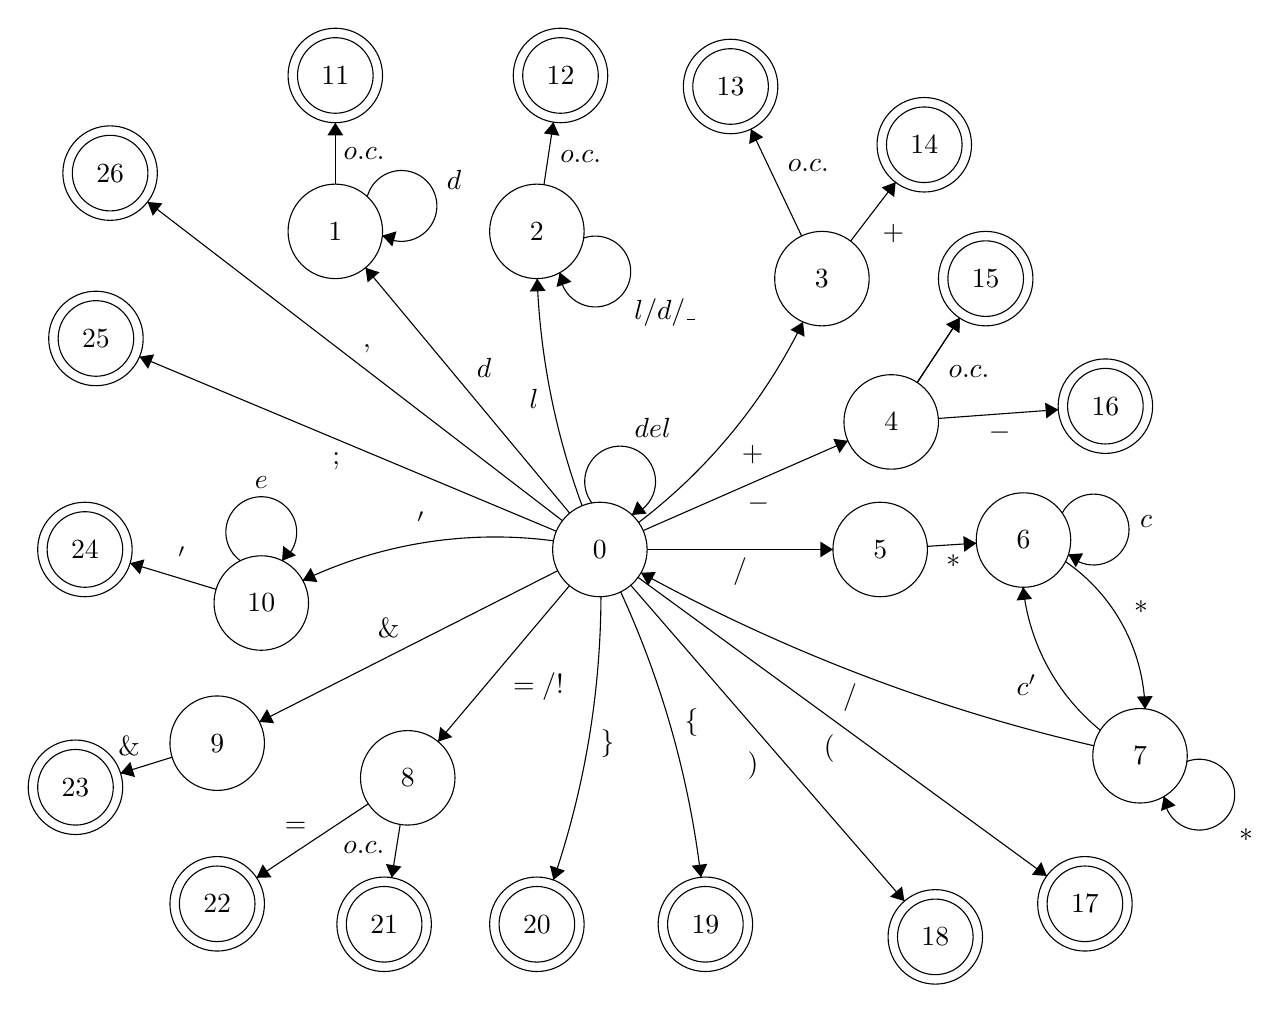
\begin{tikzpicture}[scale=0.2]
\tikzstyle{every node}+=[inner sep=0pt]
\draw [black] (38.3,-32.6) circle (3);
\draw (38.3,-32.6) node {$0$};
\draw [black] (21.5,-12.4) circle (3);
\draw (21.5,-12.4) node {$1$};
\draw [black] (21.5,-2.5) circle (3);
\draw (21.5,-2.5) node {$11$};
\draw [black] (21.5,-2.5) circle (2.4);
\draw [black] (34.3,-12.4) circle (3);
\draw (34.3,-12.4) node {$2$};
\draw [black] (35.8,-2.5) circle (3);
\draw (35.8,-2.5) node {$12$};
\draw [black] (35.8,-2.5) circle (2.4);
\draw [black] (52.4,-15.4) circle (3);
\draw (52.4,-15.4) node {$3$};
\draw [black] (46.6,-3.2) circle (3);
\draw (46.6,-3.2) node {$13$};
\draw [black] (46.6,-3.2) circle (2.4);
\draw [black] (58.9,-6.9) circle (3);
\draw (58.9,-6.9) node {$14$};
\draw [black] (58.9,-6.9) circle (2.4);
\draw [black] (56.8,-24.5) circle (3);
\draw (56.8,-24.5) node {$4$};
\draw [black] (62.8,-15.4) circle (3);
\draw (62.8,-15.4) node {$15$};
\draw [black] (62.8,-15.4) circle (2.4);
\draw [black] (70.4,-23.5) circle (3);
\draw (70.4,-23.5) node {$16$};
\draw [black] (70.4,-23.5) circle (2.4);
\draw [black] (56.1,-32.6) circle (3);
\draw (56.1,-32.6) node {$5$};
\draw [black] (72.6,-45.7) circle (3);
\draw (72.6,-45.7) node {$7$};
\draw [black] (65.2,-32) circle (3);
\draw (65.2,-32) node {$6$};
\draw [black] (69.1,-55.1) circle (3);
\draw (69.1,-55.1) node {$17$};
\draw [black] (69.1,-55.1) circle (2.4);
\draw [black] (59.6,-57.2) circle (3);
\draw (59.6,-57.2) node {$18$};
\draw [black] (59.6,-57.2) circle (2.4);
\draw [black] (45,-56.4) circle (3);
\draw (45,-56.4) node {$19$};
\draw [black] (45,-56.4) circle (2.4);
\draw [black] (34.3,-56.4) circle (3);
\draw (34.3,-56.4) node {$20$};
\draw [black] (34.3,-56.4) circle (2.4);
\draw [black] (26.1,-47.1) circle (3);
\draw (26.1,-47.1) node {$8$};
\draw [black] (24.6,-56.4) circle (3);
\draw (24.6,-56.4) node {$21$};
\draw [black] (24.6,-56.4) circle (2.4);
\draw [black] (14,-55.1) circle (3);
\draw (14,-55.1) node {$22$};
\draw [black] (14,-55.1) circle (2.4);
\draw [black] (14,-44.9) circle (3);
\draw (14,-44.9) node {$9$};
\draw [black] (5,-47.7) circle (3);
\draw (5,-47.7) node {$23$};
\draw [black] (5,-47.7) circle (2.4);
\draw [black] (16.8,-36) circle (3);
\draw (16.8,-36) node {$10$};
\draw [black] (5.6,-32.6) circle (3);
\draw (5.6,-32.6) node {$24$};
\draw [black] (5.6,-32.6) circle (2.4);
\draw [black] (6.3,-19.2) circle (3);
\draw (6.3,-19.2) node {$25$};
\draw [black] (6.3,-19.2) circle (2.4);
\draw [black] (7.2,-8.7) circle (3);
\draw (7.2,-8.7) node {$26$};
\draw [black] (7.2,-8.7) circle (2.4);
\draw [black] (37.799,-29.654) arc (217.38765:-70.61235:2.25);
\draw (41.66,-25.55) node [above] {$del$};
\fill [black] (40.33,-30.41) -- (41.27,-30.32) -- (40.67,-29.53);
\draw [black] (36.38,-30.29) -- (23.42,-14.71);
\fill [black] (23.42,-14.71) -- (23.55,-15.64) -- (24.31,-15);
\draw (30.45,-21.06) node [right] {$d$};
\draw [black] (23.526,-10.204) arc (165.03751:-122.96249:2.25);
\draw (28.55,-9.13) node [right] {$d$};
\fill [black] (24.48,-12.67) -- (25.12,-13.36) -- (25.38,-12.4);
\draw [black] (21.5,-9.4) -- (21.5,-5.5);
\fill [black] (21.5,-5.5) -- (21,-6.3) -- (22,-6.3);
\draw (22,-7.45) node [right] {$o.c.$};
\draw [black] (37.172,-29.821) arc (-159.74651:-177.85189:46.718);
\fill [black] (34.32,-15.4) -- (33.85,-16.22) -- (34.85,-16.18);
\draw (34.44,-23.03) node [left] {$l$};
\draw [black] (37.257,-12.828) arc (109.49148:-178.50852:2.25);
\draw (40.46,-17.58) node [right] {$l/d/\_$};
\fill [black] (35.76,-15.01) -- (35.55,-15.93) -- (36.5,-15.6);
\draw [black] (34.75,-9.43) -- (35.35,-5.47);
\fill [black] (35.35,-5.47) -- (34.74,-6.18) -- (35.73,-6.33);
\draw (35.75,-7.64) node [right] {$o.c.$};
\draw [black] (51.201,-18.149) arc (-25.98226:-52.70531:35.631);
\fill [black] (51.2,-18.15) -- (50.4,-18.65) -- (51.3,-19.09);
\draw (47.28,-26.56) node [right] {$+$};
\draw [black] (51.11,-12.69) -- (47.89,-5.91);
\fill [black] (47.89,-5.91) -- (47.78,-6.85) -- (48.68,-6.42);
\draw (50.21,-8.24) node [right] {$o.c.$};
\draw [black] (54.22,-13.02) -- (57.08,-9.28);
\fill [black] (57.08,-9.28) -- (56.19,-9.61) -- (56.99,-10.22);
\draw (56.22,-12.56) node [right] {$+$};
\draw [black] (41.05,-31.4) -- (54.05,-25.7);
\fill [black] (54.05,-25.7) -- (53.12,-25.57) -- (53.52,-26.48);
\draw (48.36,-29.06) node [below] {$-$};
\draw [black] (58.45,-22) -- (61.15,-17.9);
\fill [black] (61.15,-17.9) -- (60.29,-18.3) -- (61.13,-18.85);
\draw (60.41,-21.28) node [right] {$o.c.$};
\draw [black] (59.79,-24.28) -- (67.41,-23.72);
\fill [black] (67.41,-23.72) -- (66.57,-23.28) -- (66.65,-24.28);
\draw (63.69,-24.55) node [below] {$-$};
\draw [black] (58.45,-22) -- (61.15,-17.9);
\fill [black] (61.15,-17.9) -- (60.29,-18.3) -- (61.13,-18.85);
\draw [black] (41.3,-32.6) -- (53.1,-32.6);
\fill [black] (53.1,-32.6) -- (52.3,-32.1) -- (52.3,-33.1);
\draw (47.2,-33.1) node [below] {$/$};
\draw [black] (59.09,-32.4) -- (62.21,-32.2);
\fill [black] (62.21,-32.2) -- (61.38,-31.75) -- (61.44,-32.75);
\draw (60.74,-32.86) node [below] {$*$};
\draw [black] (67.655,-30.296) arc (152.4872:-135.5128:2.25);
\draw (72.57,-30.82) node [right] {$c$};
\fill [black] (68.05,-32.91) -- (68.52,-33.73) -- (68.99,-32.84);
\draw [black] (67.862,-33.365) arc (55.48576:1.26528:11.672);
\fill [black] (72.92,-42.73) -- (73.4,-41.91) -- (72.4,-41.94);
\draw (72.19,-36.26) node [right] {$*$};
\draw [black] (70.082,-44.08) arc (-129.12273:-174.12623:13.492);
\fill [black] (65.17,-34.99) -- (64.76,-35.84) -- (65.75,-35.74);
\draw (66.05,-41.2) node [left] {$c'$};
\draw [black] (75.566,-46.065) arc (110.70899:-177.29101:2.25);
\draw (78.86,-50.73) node [right] {$*$};
\fill [black] (74.11,-48.28) -- (73.93,-49.2) -- (74.86,-48.85);
\draw [black] (69.669,-45.062) arc (-103.03812:-118.76801:112.485);
\fill [black] (40.91,-34.08) -- (41.37,-34.9) -- (41.85,-34.03);
\draw (54.18,-41.08) node [below] {$/$};
\draw [black] (40.72,-34.37) -- (66.68,-53.33);
\fill [black] (66.68,-53.33) -- (66.33,-52.45) -- (65.74,-53.26);
\draw (52.86,-44.35) node [below] {$($};
\draw [black] (40.26,-34.87) -- (57.64,-54.93);
\fill [black] (57.64,-54.93) -- (57.49,-54) -- (56.73,-54.65);
\draw (48.4,-46.35) node [left] {$)$};
\draw [black] (39.62,-35.293) arc (24.69069:6.75447:60.378);
\fill [black] (44.72,-53.41) -- (45.12,-52.56) -- (44.13,-52.68);
\draw (43.65,-43.6) node [right] {$\{$};
\draw [black] (38.369,-35.599) arc (-0.2015:-18.87926:56.208);
\fill [black] (35.35,-53.59) -- (36.08,-52.99) -- (35.13,-52.67);
\draw (38.31,-44.95) node [right] {$\}$};
\draw [black] (36.37,-34.9) -- (28.03,-44.8);
\fill [black] (28.03,-44.8) -- (28.93,-44.51) -- (28.16,-43.87);
\draw (32.75,-41.29) node [right] {$=/!$};
\draw [black] (25.62,-50.06) -- (25.08,-53.44);
\fill [black] (25.08,-53.44) -- (25.7,-52.73) -- (24.71,-52.57);
\draw (24.64,-51.54) node [left] {$o.c.$};
\draw [black] (23.6,-48.75) -- (16.5,-53.45);
\fill [black] (16.5,-53.45) -- (17.45,-53.42) -- (16.89,-52.59);
\draw (18.98,-50.6) node [above] {$=$};
\draw [black] (35.62,-33.95) -- (16.68,-43.55);
\fill [black] (16.68,-43.55) -- (17.62,-43.63) -- (17.16,-42.74);
\draw (24.88,-38.24) node [above] {$\&$};
\draw [black] (11.14,-45.79) -- (7.86,-46.81);
\fill [black] (7.86,-46.81) -- (8.78,-47.05) -- (8.48,-46.09);
\draw (8.41,-45.74) node [above] {$\&$};
\draw [black] (19.434,-34.567) arc (115.50813:82.4645:28.335);
\fill [black] (19.43,-34.57) -- (20.37,-34.67) -- (19.94,-33.77);
\draw (26.94,-31.59) node [above] {$'$};
\draw [black] (15.477,-33.32) arc (234:-54:2.25);
\draw (16.8,-28.75) node [above] {$e$};
\fill [black] (18.12,-33.32) -- (19,-32.97) -- (18.19,-32.38);
\draw [black] (13.93,-35.13) -- (8.47,-33.47);
\fill [black] (8.47,-33.47) -- (9.09,-34.18) -- (9.38,-33.23);
\draw (11.77,-33.77) node [above] {$'$};
\draw [black] (35.53,-31.44) -- (9.07,-20.36);
\fill [black] (9.07,-20.36) -- (9.61,-21.13) -- (10,-20.21);
\draw (21.55,-26.41) node [below] {$;$};
\draw [black] (35.92,-30.77) -- (9.58,-10.53);
\fill [black] (9.58,-10.53) -- (9.91,-11.41) -- (10.52,-10.62);
\draw (23.51,-20.15) node [above] {$,$};
\end{tikzpicture}
\end{center}
\vspace{2cm}

\begin{center}
ACCIONES SEMÁNTICAS\\
\end{center}
\vspace{2cm}

\noindent
\textbf{Leer:}Se lee en todos los estados menos en los que pone o.c.\\
\textbf{Errores}:  Cualquier transicion no declarada dara error.\\

\textbf{Caso 0-1:}
\begin{verbatim}
    if siguienteCaracter==d
        numero=valor(d)
    else
        Error("SIMBOLO NO RECONOCIDO")
\end{verbatim}

\textbf{Caso 1-1:}
\begin{verbatim}
    if siguienteCaracter==d
        numero=numero+d
    else 
        Error("SIMBOLO NO RECONOCIDO")
\end{verbatim}

\textbf{Caso 1-11:}
\begin{verbatim}
    GenerarToken(wholeConst,numero)
\end{verbatim}

\textbf{Caso 0-2:}
\begin{verbatim}
    if siguienteCaracter==l 
        lexema=l
    else 
        Error("SIMBOLO NO RECONOCIDO")
\end{verbatim}

\textbf{Caso 2-2:}
\begin{verbatim}
    if siguienteCaracter== l | d | '_' 
        lexema=lexema+(l|d|'_')
    else 
        Error("SIMBOLO NO RECONOCIDO")
\end{verbatim}

\textbf{Caso 2-12:}
\begin{verbatim}
    GenerarToken(ID,posicionTablaSimbolos)
\end{verbatim}

\textbf{Caso 0-3:}
\begin{verbatim}
    if siguienteCaracter=='+'
        //Nada
    else
        Error("SIMBOLO NO RECONOCIDO")
\end{verbatim}

\textbf{Caso 3-13:}
\begin{verbatim}
    GenerarToken(aritOp,plus)
\end{verbatim}

\textbf{Caso 3-14:}
\begin{verbatim}
    if siguienteCaracter=='+'
        GenerarToken(autoIncOp,autoinc)
    else 
        Error("SIMBOLO NO RECONOCIDO")
\end{verbatim}

\textbf{Caso 0-4:}
\begin{verbatim}
    if siguienteCaracter=='-'
        //Nada
    else
        Error("SIMBOLO NO RECONOCIDO")
\end{verbatim}

\textbf{Caso 4-15:}
\begin{verbatim}
    GenerarToken(aritOp,minus)
\end{verbatim}

\textbf{Caso 4-16:}
\begin{verbatim}
    if siguienteCarcter=='-'
        GenerarToken(autoIncOp,autoinc)
    else 
        Error("SIMBOLO NO RECONOCIDO")
\end{verbatim}

\textbf{Caso 0-5:}
\begin{verbatim}
    if siguienteCaracter=='/'
        //NADA
    else
        Error("SIMBOLO NO RECONOCIDO")
\end{verbatim}

\textbf{Caso 5-6:}
\begin{verbatim}
    if siguienteCaracater=='*'
        //NADA
    else
        Error("SIMBOLO NO RECONOCIDO")
\end{verbatim}

\textbf{Caso 6-6:}
\begin{verbatim}
    if siguienteCaracater=='c'
        //NADA
    else
        Error("SIMBOLO NO RECONOCIDO")
\end{verbatim}

\textbf{Caso 6-7:}
\begin{verbatim}
    if siguienteCaracater=='*'
         //NADA
    else
         Error("SIMBOLO NO RECONOCIDO")
\end{verbatim}

\textbf{Caso 7-6:}
\begin{verbatim}
    if siguienteCaracater=='c''
        //NADA
    else
        Error("SIMBOLO NO RECONOCIDO")
\end{verbatim}

\textbf{Caso 7-0:}
\begin{verbatim}
    if siguienteCaracater=='/'
        //NADA
    else
        Error("SIMBOLO NO RECONOCIDO")
\end{verbatim}

\textbf{Caso 0-26:}
\begin{verbatim}
    if siguienteCaracter==','
        GenerarToken(separator,colon)
    else
        Error("SIMBOLO NO RECONOCIDO")
\end{verbatim}

\textbf{Caso 0-25:}
\begin{verbatim}
    if siguienteCaracter==';'
        GenerarToken(separator,semicolon)
    else
        Error("SIMBOLO NO RECONOCIDO") )
\end{verbatim}

\textbf{Caso 0-20:}
\begin{verbatim}
    if siguienteCaracter=='}'
        GenerarToken(separator,closeBraq)
    else
        Error("SIMBOLO NO RECONOCIDO")  
\end{verbatim}

\textbf{Caso 0-19:}
\begin{verbatim}
    if siguienteCaracter=='{'
        GenerarToken(separator,openBraq)
    else
        Error("SIMBOLO NO RECONOCIDO")
\end{verbatim}

\textbf{Caso 0-18:}
\begin{verbatim}
    if siguienteCaracter==')'
        GenerarToken(separator,closePar)
    else
        Error("SIMBOLO NO RECONOCIDO")  
\end{verbatim}

\textbf{Caso 0-17:}
\begin{verbatim}
    if siguienteCaracter=='('
        GenerarToken(separator,openPar)
    else
        Error("SIMBOLO NO RECONOCIDO")
\end{verbatim}

\textbf{Caso 0-10:}
\begin{verbatim}
    if siguienteCaracter=='''
        lexema=''
    else
        Error ("SIMBOLO NO RECONOCIDO)
\end{verbatim}

\textbf{Caso 10-10:}
\begin{verbatim}
    if siguienteCaracter==e
        lexema=lexema+e
    else 
        Error ("SIMBOLO NO RECONOCIDO)
\end{verbatim}

\textbf{Caso 10-24:}
\begin{verbatim}
    if siguienteCaracater=='''
        GenerarToken(chain,posicionTablaSimbolos)//revisar
    else 
        Error ("SIMBOLO NO RECONOCIDO)
\end{verbatim}

\textbf{Caso 0-8:}
\begin{verbatim}
    if siguienteCaracter=='='

    else if siguienteCaracater=='!'
    
    else 
        Error ("SIMBOLO NO RECONOCIDO")
\end{verbatim}

\textbf{Caso 8-22:}
\begin{verbatim}
    if siguienteCaracater == '='
        GenerarToken(relOp,equals)
    else 
        Error ("SIMBOLO NO RECONOCIDO")  
\end{verbatim}






\end{document}